\documentclass[]{article}
\usepackage{lmodern}
\usepackage{amssymb,amsmath}
\usepackage{ifxetex,ifluatex}
\usepackage{fixltx2e} % provides \textsubscript
\ifnum 0\ifxetex 1\fi\ifluatex 1\fi=0 % if pdftex
  \usepackage[T1]{fontenc}
  \usepackage[utf8]{inputenc}
\else % if luatex or xelatex
  \ifxetex
    \usepackage{mathspec}
  \else
    \usepackage{fontspec}
  \fi
  \defaultfontfeatures{Ligatures=TeX,Scale=MatchLowercase}
\fi
% use upquote if available, for straight quotes in verbatim environments
\IfFileExists{upquote.sty}{\usepackage{upquote}}{}
% use microtype if available
\IfFileExists{microtype.sty}{%
\usepackage{microtype}
\UseMicrotypeSet[protrusion]{basicmath} % disable protrusion for tt fonts
}{}
\usepackage[margin=1in]{geometry}
\usepackage{hyperref}
\hypersetup{unicode=true,
            pdftitle={sample},
            pdfborder={0 0 0},
            breaklinks=true}
\urlstyle{same}  % don't use monospace font for urls
\usepackage{color}
\usepackage{fancyvrb}
\newcommand{\VerbBar}{|}
\newcommand{\VERB}{\Verb[commandchars=\\\{\}]}
\DefineVerbatimEnvironment{Highlighting}{Verbatim}{commandchars=\\\{\}}
% Add ',fontsize=\small' for more characters per line
\usepackage{framed}
\definecolor{shadecolor}{RGB}{248,248,248}
\newenvironment{Shaded}{\begin{snugshade}}{\end{snugshade}}
\newcommand{\AlertTok}[1]{\textcolor[rgb]{0.94,0.16,0.16}{#1}}
\newcommand{\AnnotationTok}[1]{\textcolor[rgb]{0.56,0.35,0.01}{\textbf{\textit{#1}}}}
\newcommand{\AttributeTok}[1]{\textcolor[rgb]{0.77,0.63,0.00}{#1}}
\newcommand{\BaseNTok}[1]{\textcolor[rgb]{0.00,0.00,0.81}{#1}}
\newcommand{\BuiltInTok}[1]{#1}
\newcommand{\CharTok}[1]{\textcolor[rgb]{0.31,0.60,0.02}{#1}}
\newcommand{\CommentTok}[1]{\textcolor[rgb]{0.56,0.35,0.01}{\textit{#1}}}
\newcommand{\CommentVarTok}[1]{\textcolor[rgb]{0.56,0.35,0.01}{\textbf{\textit{#1}}}}
\newcommand{\ConstantTok}[1]{\textcolor[rgb]{0.00,0.00,0.00}{#1}}
\newcommand{\ControlFlowTok}[1]{\textcolor[rgb]{0.13,0.29,0.53}{\textbf{#1}}}
\newcommand{\DataTypeTok}[1]{\textcolor[rgb]{0.13,0.29,0.53}{#1}}
\newcommand{\DecValTok}[1]{\textcolor[rgb]{0.00,0.00,0.81}{#1}}
\newcommand{\DocumentationTok}[1]{\textcolor[rgb]{0.56,0.35,0.01}{\textbf{\textit{#1}}}}
\newcommand{\ErrorTok}[1]{\textcolor[rgb]{0.64,0.00,0.00}{\textbf{#1}}}
\newcommand{\ExtensionTok}[1]{#1}
\newcommand{\FloatTok}[1]{\textcolor[rgb]{0.00,0.00,0.81}{#1}}
\newcommand{\FunctionTok}[1]{\textcolor[rgb]{0.00,0.00,0.00}{#1}}
\newcommand{\ImportTok}[1]{#1}
\newcommand{\InformationTok}[1]{\textcolor[rgb]{0.56,0.35,0.01}{\textbf{\textit{#1}}}}
\newcommand{\KeywordTok}[1]{\textcolor[rgb]{0.13,0.29,0.53}{\textbf{#1}}}
\newcommand{\NormalTok}[1]{#1}
\newcommand{\OperatorTok}[1]{\textcolor[rgb]{0.81,0.36,0.00}{\textbf{#1}}}
\newcommand{\OtherTok}[1]{\textcolor[rgb]{0.56,0.35,0.01}{#1}}
\newcommand{\PreprocessorTok}[1]{\textcolor[rgb]{0.56,0.35,0.01}{\textit{#1}}}
\newcommand{\RegionMarkerTok}[1]{#1}
\newcommand{\SpecialCharTok}[1]{\textcolor[rgb]{0.00,0.00,0.00}{#1}}
\newcommand{\SpecialStringTok}[1]{\textcolor[rgb]{0.31,0.60,0.02}{#1}}
\newcommand{\StringTok}[1]{\textcolor[rgb]{0.31,0.60,0.02}{#1}}
\newcommand{\VariableTok}[1]{\textcolor[rgb]{0.00,0.00,0.00}{#1}}
\newcommand{\VerbatimStringTok}[1]{\textcolor[rgb]{0.31,0.60,0.02}{#1}}
\newcommand{\WarningTok}[1]{\textcolor[rgb]{0.56,0.35,0.01}{\textbf{\textit{#1}}}}
\usepackage{graphicx,grffile}
\makeatletter
\def\maxwidth{\ifdim\Gin@nat@width>\linewidth\linewidth\else\Gin@nat@width\fi}
\def\maxheight{\ifdim\Gin@nat@height>\textheight\textheight\else\Gin@nat@height\fi}
\makeatother
% Scale images if necessary, so that they will not overflow the page
% margins by default, and it is still possible to overwrite the defaults
% using explicit options in \includegraphics[width, height, ...]{}
\setkeys{Gin}{width=\maxwidth,height=\maxheight,keepaspectratio}
\IfFileExists{parskip.sty}{%
\usepackage{parskip}
}{% else
\setlength{\parindent}{0pt}
\setlength{\parskip}{6pt plus 2pt minus 1pt}
}
\setlength{\emergencystretch}{3em}  % prevent overfull lines
\providecommand{\tightlist}{%
  \setlength{\itemsep}{0pt}\setlength{\parskip}{0pt}}
\setcounter{secnumdepth}{0}
% Redefines (sub)paragraphs to behave more like sections
\ifx\paragraph\undefined\else
\let\oldparagraph\paragraph
\renewcommand{\paragraph}[1]{\oldparagraph{#1}\mbox{}}
\fi
\ifx\subparagraph\undefined\else
\let\oldsubparagraph\subparagraph
\renewcommand{\subparagraph}[1]{\oldsubparagraph{#1}\mbox{}}
\fi

%%% Use protect on footnotes to avoid problems with footnotes in titles
\let\rmarkdownfootnote\footnote%
\def\footnote{\protect\rmarkdownfootnote}

%%% Change title format to be more compact
\usepackage{titling}

% Create subtitle command for use in maketitle
\providecommand{\subtitle}[1]{
  \posttitle{
    \begin{center}\large#1\end{center}
    }
}

\setlength{\droptitle}{-2em}

  \title{sample}
    \pretitle{\vspace{\droptitle}\centering\huge}
  \posttitle{\par}
    \author{}
    \preauthor{}\postauthor{}
    \date{}
    \predate{}\postdate{}
  

\begin{document}
\maketitle

시작전

\begin{Shaded}
\begin{Highlighting}[]
\KeywordTok{library}\NormalTok{(ggplot2)}
\end{Highlighting}
\end{Shaded}

\begin{verbatim}
## Registered S3 methods overwritten by 'ggplot2':
##   method         from 
##   [.quosures     rlang
##   c.quosures     rlang
##   print.quosures rlang
\end{verbatim}

\begin{Shaded}
\begin{Highlighting}[]
\KeywordTok{library}\NormalTok{(googleVis)}
\end{Highlighting}
\end{Shaded}

\begin{verbatim}
## Creating a generic function for 'toJSON' from package 'jsonlite' in package 'googleVis'
\end{verbatim}

\begin{verbatim}
## 
## Welcome to googleVis version 0.6.4
## 
## Please read Google's Terms of Use
## before you start using the package:
## https://developers.google.com/terms/
## 
## Note, the plot method of googleVis will by default use
## the standard browser to display its output.
## 
## See the googleVis package vignettes for more details,
## or visit https://github.com/mages/googleVis.
## 
## To suppress this message use:
## suppressPackageStartupMessages(library(googleVis))
\end{verbatim}

\begin{Shaded}
\begin{Highlighting}[]
\KeywordTok{library}\NormalTok{(plyr)}
\KeywordTok{library}\NormalTok{(dplyr)}
\end{Highlighting}
\end{Shaded}

\begin{verbatim}
## 
## Attaching package: 'dplyr'
\end{verbatim}

\begin{verbatim}
## The following objects are masked from 'package:plyr':
## 
##     arrange, count, desc, failwith, id, mutate, rename, summarise,
##     summarize
\end{verbatim}

\begin{verbatim}
## The following objects are masked from 'package:stats':
## 
##     filter, lag
\end{verbatim}

\begin{verbatim}
## The following objects are masked from 'package:base':
## 
##     intersect, setdiff, setequal, union
\end{verbatim}

\begin{enumerate}
\def\labelenumi{\arabic{enumi}.}
\tightlist
\item
  mpg 데이터의 cty(도시 연비)와 hwy(고속도로 연비) 간에 어떤 관계가
  있는지 알아보려고 합니다. x축은 cty, y축은 hwy로 된 산점도를 만들어
  보세요
\end{enumerate}

\begin{Shaded}
\begin{Highlighting}[]
\NormalTok{mpg}
\end{Highlighting}
\end{Shaded}

\begin{verbatim}
## # A tibble: 234 x 11
##    manufacturer model displ  year   cyl trans drv     cty   hwy fl    class
##    <chr>        <chr> <dbl> <int> <int> <chr> <chr> <int> <int> <chr> <chr>
##  1 audi         a4      1.8  1999     4 auto~ f        18    29 p     comp~
##  2 audi         a4      1.8  1999     4 manu~ f        21    29 p     comp~
##  3 audi         a4      2    2008     4 manu~ f        20    31 p     comp~
##  4 audi         a4      2    2008     4 auto~ f        21    30 p     comp~
##  5 audi         a4      2.8  1999     6 auto~ f        16    26 p     comp~
##  6 audi         a4      2.8  1999     6 manu~ f        18    26 p     comp~
##  7 audi         a4      3.1  2008     6 auto~ f        18    27 p     comp~
##  8 audi         a4 q~   1.8  1999     4 manu~ 4        18    26 p     comp~
##  9 audi         a4 q~   1.8  1999     4 auto~ 4        16    25 p     comp~
## 10 audi         a4 q~   2    2008     4 manu~ 4        20    28 p     comp~
## # ... with 224 more rows
\end{verbatim}

\begin{Shaded}
\begin{Highlighting}[]
\NormalTok{data <-}\StringTok{ }\NormalTok{mpg}

\KeywordTok{ggplot}\NormalTok{(data, }\KeywordTok{aes}\NormalTok{(}\DataTypeTok{x =}\NormalTok{ cty, }\DataTypeTok{y =}\NormalTok{ hwy)) }\OperatorTok{+}
\StringTok{  }\KeywordTok{geom_point}\NormalTok{()}
\end{Highlighting}
\end{Shaded}

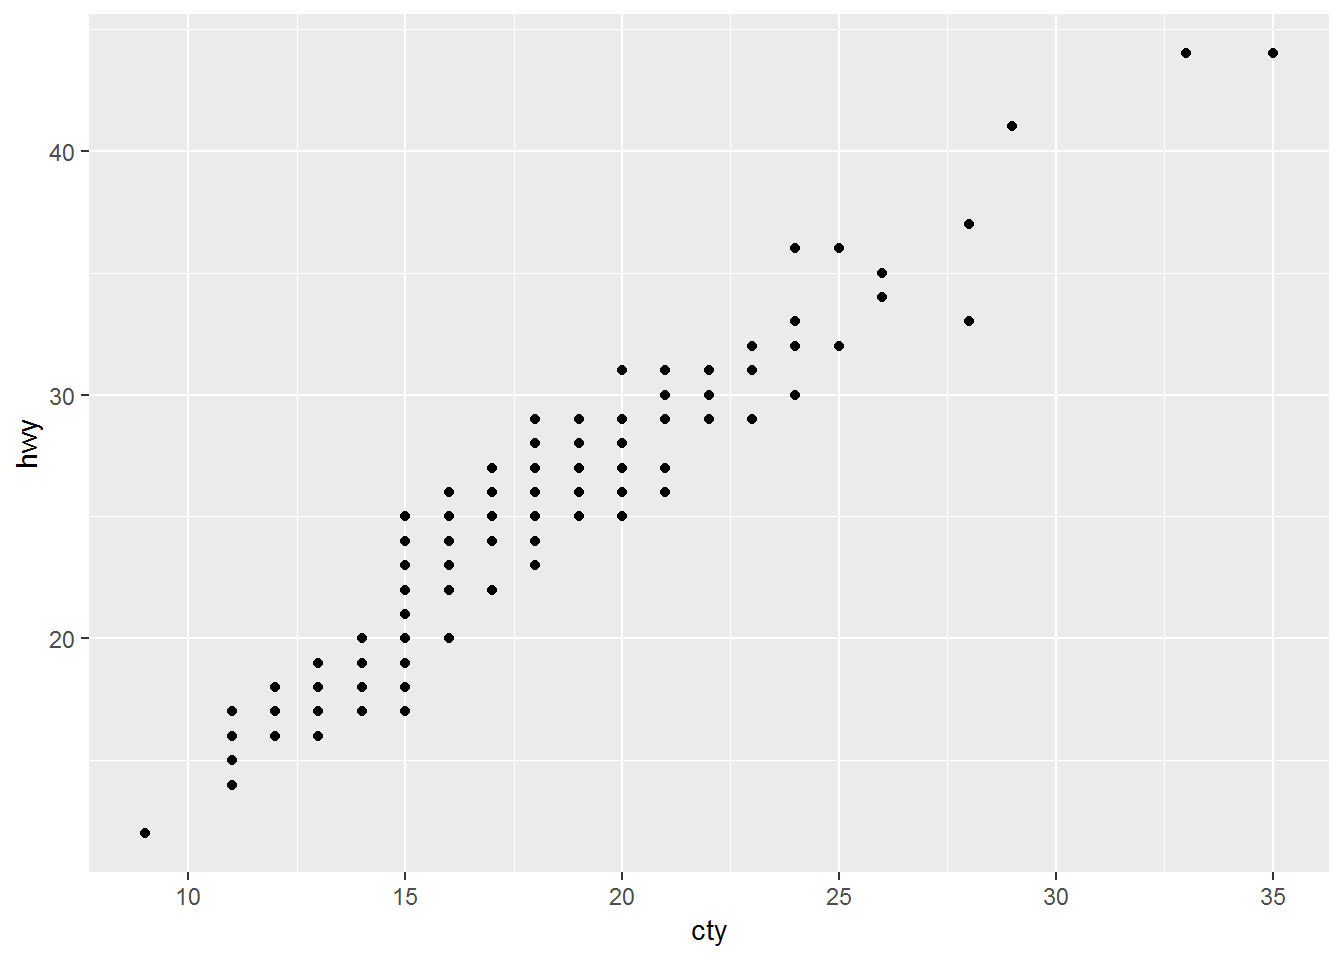
\includegraphics{jbm_files/figure-latex/unnamed-chunk-2-1.pdf}

\begin{Shaded}
\begin{Highlighting}[]
\NormalTok{asia <-}\StringTok{ }\NormalTok{midwest}
\NormalTok{asia1_}\DecValTok{1}\NormalTok{ <-}\StringTok{ }\NormalTok{asia }\OperatorTok
\StringTok{  }\KeywordTok{select}\NormalTok{(poptotal,popasian)}

\NormalTok{asia1_}\DecValTok{2}\NormalTok{ <-}\StringTok{ }\KeywordTok{filter}\NormalTok{(asia1_}\DecValTok{1}\NormalTok{, poptotal}\OperatorTok{<}\DecValTok{500000} \OperatorTok{&}\StringTok{ }\NormalTok{popasian}\OperatorTok{<=}\DecValTok{10000}\NormalTok{)}
\end{Highlighting}
\end{Shaded}

\begin{enumerate}
\def\labelenumi{\arabic{enumi}.}
\setcounter{enumi}{1}
\tightlist
\item
  미국 지역별 인구통계 정보를 담은 ggplot2 패키지의 midwest 데이터를
  이용해서 전체 인구와 아시아인 인구 간에 어떤 관계가 있는지 알아보려고
  합니다. x축은 poptotal(전체 인구), y축은 popasian(아시아인 인구)으로
  된 산점도를 만들어 보세요. 전체 인구는 50만 명 이하, 아시아인 인구는
  1만 명 이하인 지역만 산점도에 표시되게 설정하세요.
\end{enumerate}

\begin{Shaded}
\begin{Highlighting}[]
\NormalTok{asia1_}\DecValTok{2}\NormalTok{ <-}\StringTok{ }\KeywordTok{filter}\NormalTok{(asia1_}\DecValTok{1}\NormalTok{, poptotal}\OperatorTok{<}\DecValTok{500000} \OperatorTok{&}\StringTok{ }\NormalTok{popasian}\OperatorTok{<=}\DecValTok{10000}\NormalTok{)}

\KeywordTok{ggplot}\NormalTok{(asia, }\KeywordTok{aes}\NormalTok{(}\DataTypeTok{x =}\NormalTok{ poptotal, }\DataTypeTok{y=}\NormalTok{ popasian )) }\OperatorTok{+}
\StringTok{  }\KeywordTok{geom_point}\NormalTok{(}\DataTypeTok{size =} \DecValTok{1}\NormalTok{)}
\end{Highlighting}
\end{Shaded}

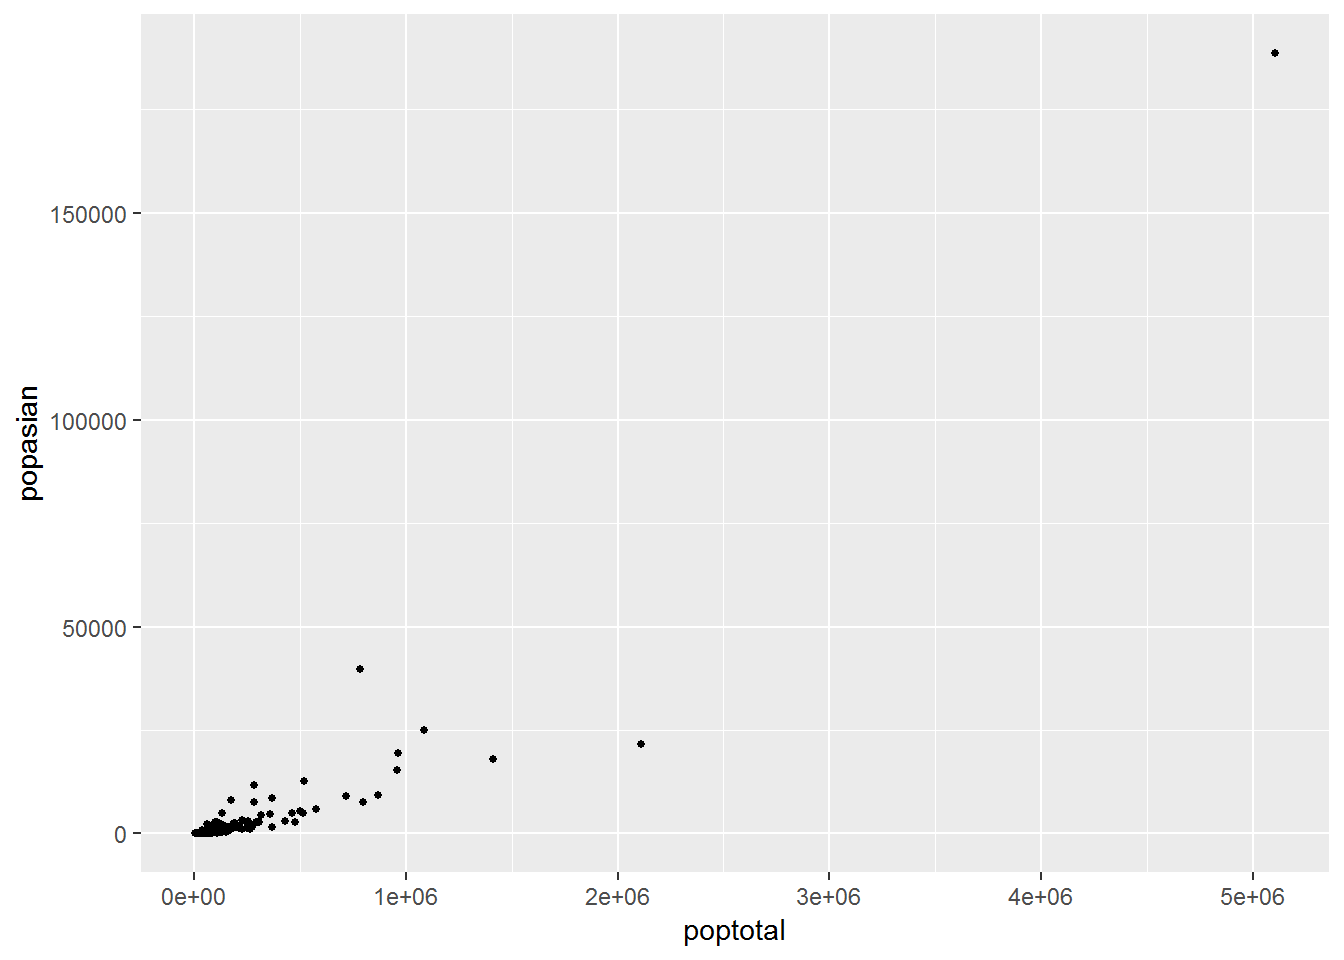
\includegraphics{jbm_files/figure-latex/unnamed-chunk-3-1.pdf}

\begin{enumerate}
\def\labelenumi{\arabic{enumi}.}
\setcounter{enumi}{2}
\tightlist
\item
  어떤 회사에서 생산한 ``suv'' 차종의 도시 연비가 높은지 알아보려고
  합니다. ``suv'' 차종을 대상으로 평균 cty(도시 연비)가 가장 높은 회사
  다섯 곳을 막대 그래프로 표현해 보세요. 막대는 연비가 높은 순으로
  정렬하세요.
\end{enumerate}

\begin{Shaded}
\begin{Highlighting}[]
\NormalTok{data1 <-}\StringTok{ }\KeywordTok{select}\NormalTok{(data, cty, class, manufacturer) }\OperatorTok
\StringTok{  }\KeywordTok{filter}\NormalTok{(class }\OperatorTok{==}\StringTok{ 'suv'}\NormalTok{)}

\NormalTok{data1 }\OperatorTok
\StringTok{  }\KeywordTok{group_by}\NormalTok{(manufacturer) }\OperatorTok
\StringTok{  }\KeywordTok{summarise}\NormalTok{(}\DataTypeTok{averge =} \KeywordTok{mean}\NormalTok{(cty,}\DataTypeTok{na.rm =} \OtherTok{TRUE}\NormalTok{)) }\OperatorTok
\StringTok{  }\KeywordTok{arrange}\NormalTok{(}\KeywordTok{desc}\NormalTok{(averge))}
\end{Highlighting}
\end{Shaded}

\begin{verbatim}
## # A tibble: 10 x 2
##    manufacturer averge
##    <chr>         <dbl>
##  1 subaru         18.8
##  2 toyota         14.4
##  3 nissan         13.8
##  4 jeep           13.5
##  5 mercury        13.2
##  6 ford           12.9
##  7 chevrolet      12.7
##  8 dodge          11.9
##  9 land rover     11.5
## 10 lincoln        11.3
\end{verbatim}

\begin{Shaded}
\begin{Highlighting}[]
\NormalTok{data1_}\DecValTok{1}\NormalTok{ <-}\StringTok{ }\NormalTok{data1 }\OperatorTok
\StringTok{  }\KeywordTok{filter}\NormalTok{(manufacturer}\OperatorTok{==}\StringTok{'subaru'} \OperatorTok{|}\StringTok{ }\NormalTok{manufacturer}\OperatorTok{==}\StringTok{'toyota'} \OperatorTok{|}\StringTok{ }
\StringTok{           }\NormalTok{manufacturer}\OperatorTok{==}\StringTok{'nissan'} \OperatorTok{|}\StringTok{ }\NormalTok{manufacturer}\OperatorTok{==}\StringTok{'jeep'} \OperatorTok{|}
\StringTok{           }\NormalTok{manufacturer}\OperatorTok{==}\StringTok{'mercury'}\NormalTok{)}

\NormalTok{data1_}\DecValTok{2}\NormalTok{ <-}\StringTok{ }\NormalTok{data1_}\DecValTok{1} \OperatorTok
\StringTok{  }\KeywordTok{group_by}\NormalTok{(manufacturer) }\OperatorTok
\StringTok{  }\KeywordTok{summarise}\NormalTok{(}\DataTypeTok{averge =} \KeywordTok{mean}\NormalTok{(cty,}\DataTypeTok{na.rm =} \OtherTok{TRUE}\NormalTok{))}

\KeywordTok{ggplot}\NormalTok{(data1_}\DecValTok{2}\NormalTok{, }\KeywordTok{aes}\NormalTok{(}\DataTypeTok{x =} \KeywordTok{reorder}\NormalTok{(manufacturer, }\OperatorTok{-}\NormalTok{data1_}\DecValTok{2}\OperatorTok{$}\NormalTok{averge), }\DataTypeTok{y=}\NormalTok{ averge)) }\OperatorTok{+}
\StringTok{         }\KeywordTok{geom_bar}\NormalTok{(}\DataTypeTok{stat=}\StringTok{'identity'}\NormalTok{)}
\end{Highlighting}
\end{Shaded}

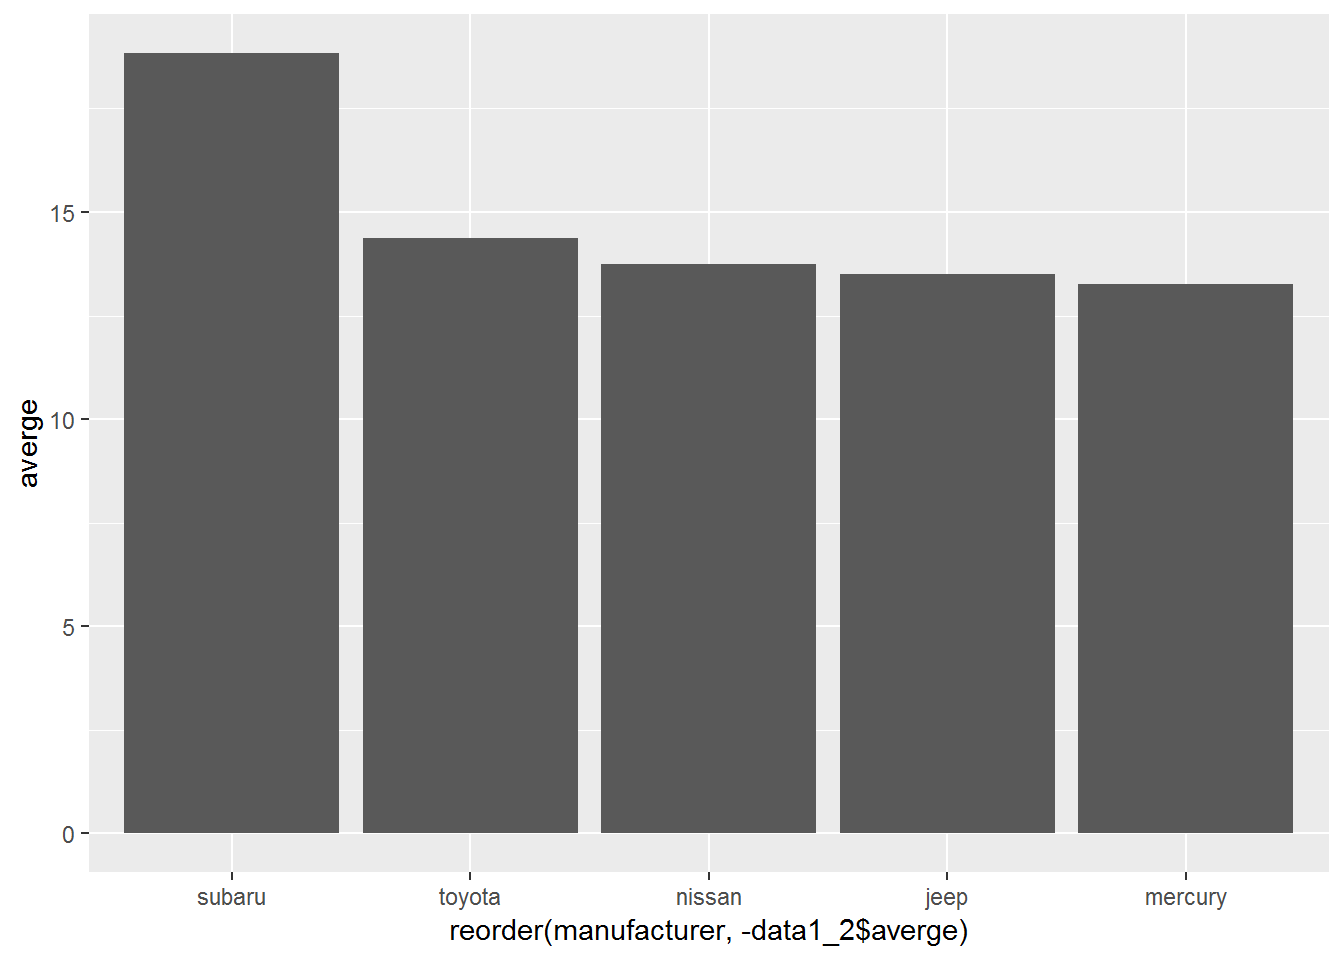
\includegraphics{jbm_files/figure-latex/unnamed-chunk-4-1.pdf}

\begin{enumerate}
\def\labelenumi{\arabic{enumi}.}
\setcounter{enumi}{3}
\tightlist
\item
  자동차 중에서 어떤 class(자동차 종류)가 가장 많은지 알아보려고 합니다.
  자동차 종류별 빈도를 표현한 막대 그래프를 만들어 보세요.
\end{enumerate}

\begin{Shaded}
\begin{Highlighting}[]
\NormalTok{data3 <-}\StringTok{ }\KeywordTok{select}\NormalTok{(data, class) }\OperatorTok
\StringTok{  }\KeywordTok{mutate}\NormalTok{(}\DataTypeTok{T =} \DecValTok{1}\NormalTok{) }\OperatorTok
\StringTok{  }\KeywordTok{group_by}\NormalTok{(class) }\OperatorTok
\StringTok{  }\KeywordTok{summarise}\NormalTok{(}\DataTypeTok{sum =} \KeywordTok{sum}\NormalTok{(T))}

\KeywordTok{ggplot}\NormalTok{(data3, }\KeywordTok{aes}\NormalTok{(}\DataTypeTok{x=}\KeywordTok{reorder}\NormalTok{(class, }\OperatorTok{-}\NormalTok{data3}\OperatorTok{$}\NormalTok{sum), }\DataTypeTok{y=}\NormalTok{sum)) }\OperatorTok{+}
\StringTok{  }\KeywordTok{geom_bar}\NormalTok{(}\DataTypeTok{stat=}\StringTok{'identity'}\NormalTok{)}
\end{Highlighting}
\end{Shaded}

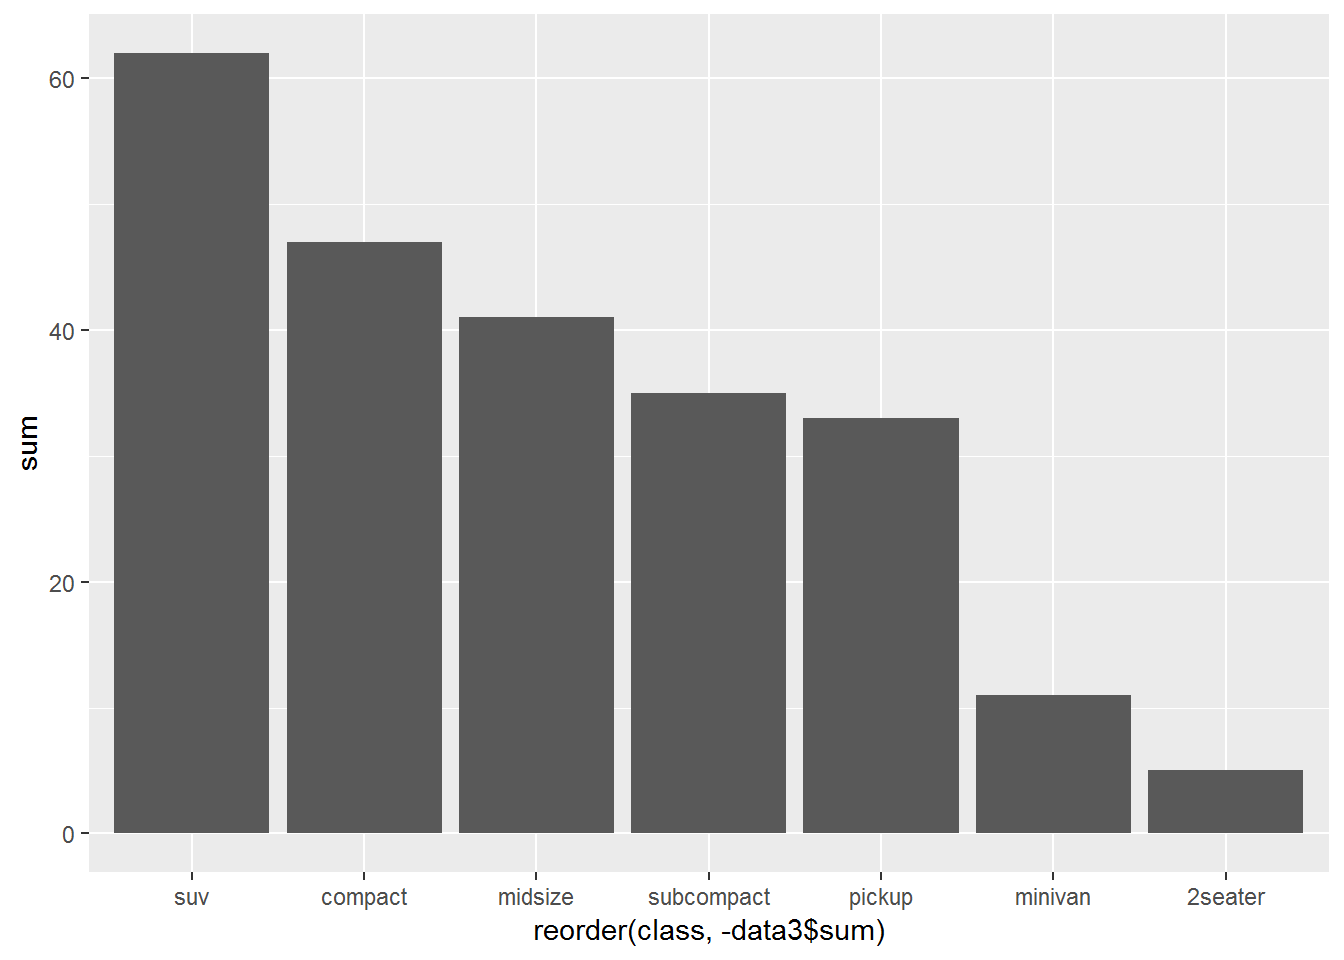
\includegraphics{jbm_files/figure-latex/unnamed-chunk-5-1.pdf}

\begin{enumerate}
\def\labelenumi{\arabic{enumi}.}
\setcounter{enumi}{4}
\tightlist
\item
  economics 데이터를 이용해서 psavert(개인 저축률)가 시간에 따라서
  어떻게 변해왔는지 알아보려고 합니다. 시간에 따른 개인 저축률의 변화를
  나타낸 시계열 그래프를 만들어 보세요.
\end{enumerate}

\begin{Shaded}
\begin{Highlighting}[]
\NormalTok{economics}
\end{Highlighting}
\end{Shaded}

\begin{verbatim}
## # A tibble: 574 x 6
##    date         pce    pop psavert uempmed unemploy
##    <date>     <dbl>  <int>   <dbl>   <dbl>    <int>
##  1 1967-07-01  507. 198712    12.5     4.5     2944
##  2 1967-08-01  510. 198911    12.5     4.7     2945
##  3 1967-09-01  516. 199113    11.7     4.6     2958
##  4 1967-10-01  513. 199311    12.5     4.9     3143
##  5 1967-11-01  518. 199498    12.5     4.7     3066
##  6 1967-12-01  526. 199657    12.1     4.8     3018
##  7 1968-01-01  532. 199808    11.7     5.1     2878
##  8 1968-02-01  534. 199920    12.2     4.5     3001
##  9 1968-03-01  545. 200056    11.6     4.1     2877
## 10 1968-04-01  545. 200208    12.2     4.6     2709
## # ... with 564 more rows
\end{verbatim}

\begin{Shaded}
\begin{Highlighting}[]
\NormalTok{data_e <-}\StringTok{ }\NormalTok{economics}

\NormalTok{data4 <-}\KeywordTok{select}\NormalTok{(data_e, psavert, date)}

\KeywordTok{ggplot}\NormalTok{(data_e, }\KeywordTok{aes}\NormalTok{(}\DataTypeTok{x=}\NormalTok{date,}\DataTypeTok{y=}\NormalTok{psavert)) }\OperatorTok{+}
\StringTok{  }\KeywordTok{geom_line}\NormalTok{()}
\end{Highlighting}
\end{Shaded}

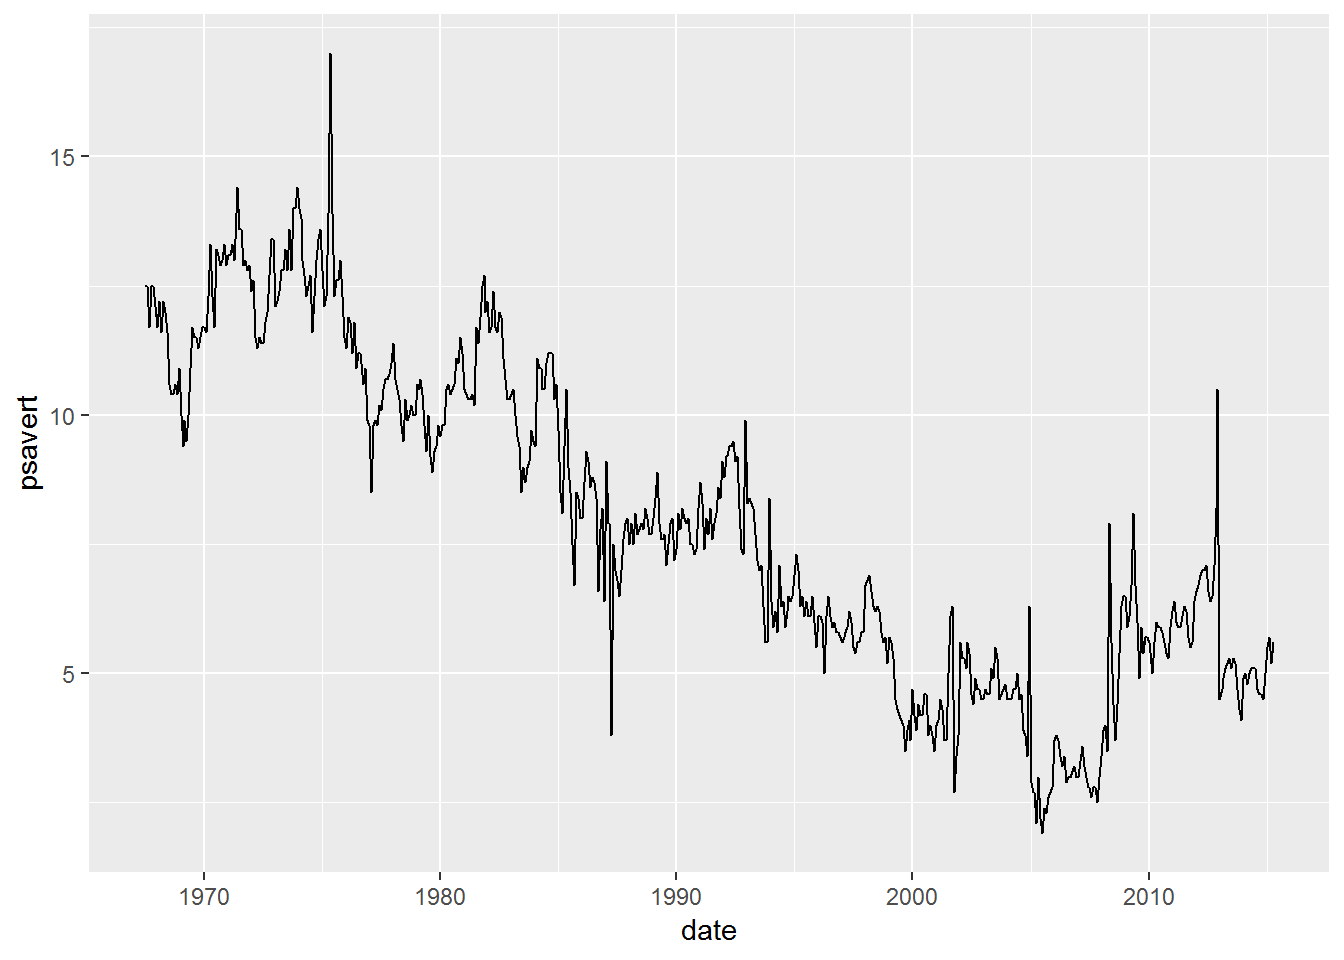
\includegraphics{jbm_files/figure-latex/unnamed-chunk-6-1.pdf}

\begin{enumerate}
\def\labelenumi{\arabic{enumi}.}
\setcounter{enumi}{5}
\tightlist
\item
  class(자동차 종류)가 ``compact'', ``subcompact'', ``suv''인 자동차의
  cty(도시 연비)가 어떻게 다른지 비교해보려고 합니다. 세 차종의 cty를
  나타낸 상자 그림을 만들어보세요.
\end{enumerate}

\begin{Shaded}
\begin{Highlighting}[]
\NormalTok{data5 <-}\StringTok{ }\KeywordTok{select}\NormalTok{(data, cty, class, manufacturer) }\OperatorTok
\StringTok{  }\KeywordTok{filter}\NormalTok{(class }\OperatorTok{==}\StringTok{ 'suv'} \OperatorTok{|}\StringTok{ }\NormalTok{class }\OperatorTok{==}\StringTok{ 'compact'} \OperatorTok{|}\StringTok{ }\NormalTok{class }\OperatorTok{==}\StringTok{ 'subcompact'}\NormalTok{)}
\CommentTok{#filter(class %in% c( 'suv','compact','subcompact')}
\KeywordTok{ggplot}\NormalTok{(data5, }\KeywordTok{aes}\NormalTok{(}\DataTypeTok{x=}\NormalTok{class, }\DataTypeTok{y=}\NormalTok{cty)) }\OperatorTok{+}
\StringTok{  }\KeywordTok{geom_boxplot}\NormalTok{()}
\end{Highlighting}
\end{Shaded}

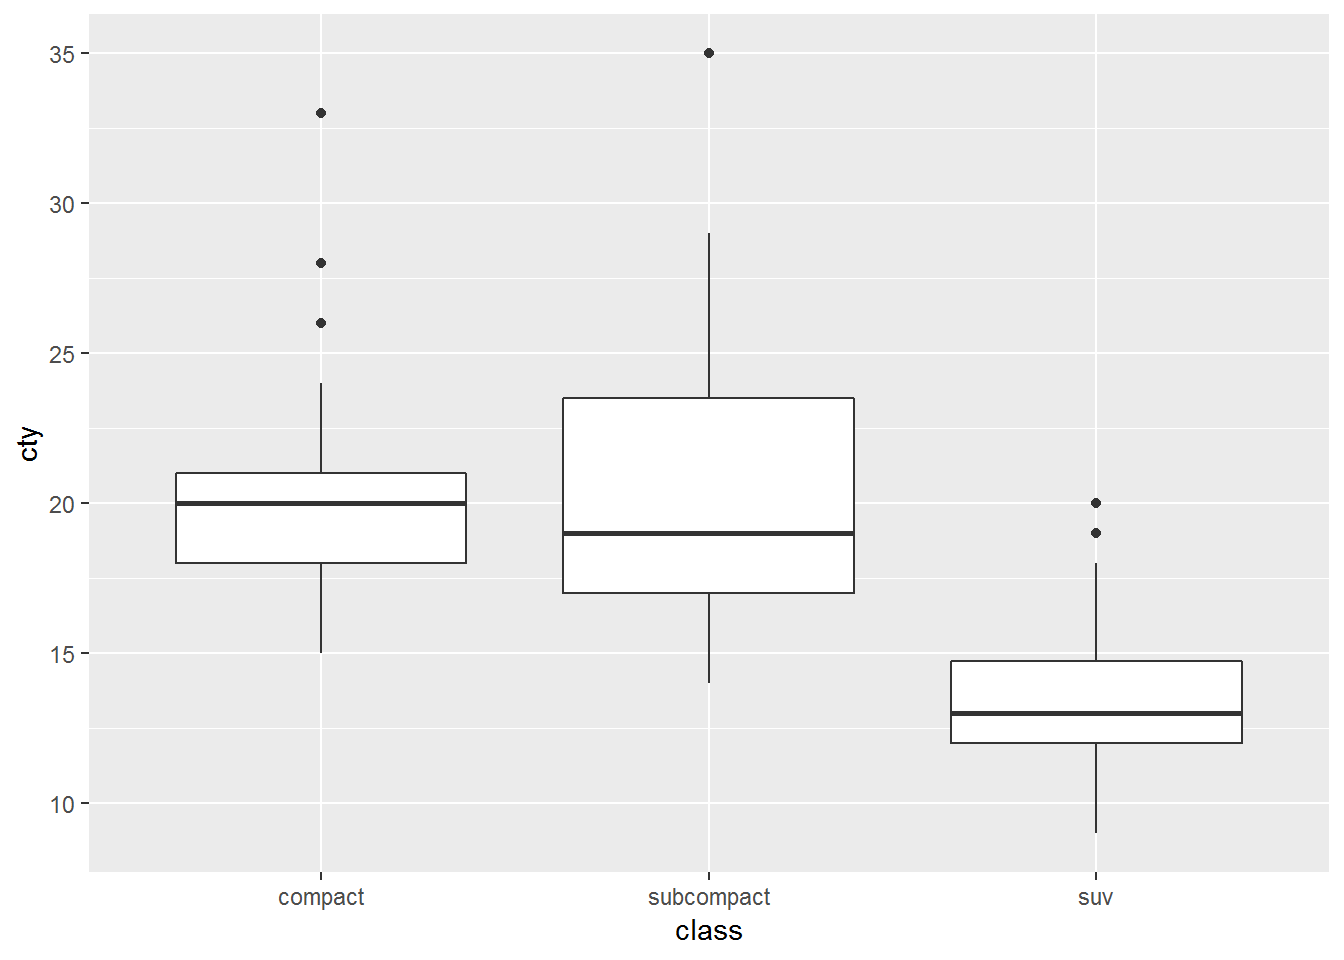
\includegraphics{jbm_files/figure-latex/unnamed-chunk-7-1.pdf}

\begin{enumerate}
\def\labelenumi{\arabic{enumi}.}
\setcounter{enumi}{6}
\tightlist
\item
  Diamonds 데이터 셋을 이용하여 다음 문제를 해결하세요. 단, 컬러, 제목,
  x축, y축 등 그래프를 예쁘게 작성하세요.
\end{enumerate}

\begin{enumerate}
\def\labelenumi{\arabic{enumi})}
\tightlist
\item
  cut의 돗수를 보여주는 그래프를 작성하세요.
\end{enumerate}

\begin{Shaded}
\begin{Highlighting}[]
\NormalTok{data6 <-}\StringTok{ }\NormalTok{diamonds}

\NormalTok{data7 <-}\StringTok{ }\KeywordTok{select}\NormalTok{(data6, cut) }\OperatorTok
\StringTok{  }\KeywordTok{mutate}\NormalTok{(}\DataTypeTok{nt =} \DecValTok{1}\NormalTok{) }\OperatorTok
\StringTok{  }\KeywordTok{group_by}\NormalTok{(cut) }\OperatorTok
\StringTok{  }\KeywordTok{summarise}\NormalTok{(}\DataTypeTok{sum =} \KeywordTok{sum}\NormalTok{(nt))}

\KeywordTok{ggplot}\NormalTok{(data7, }\KeywordTok{aes}\NormalTok{(}\DataTypeTok{x=}\NormalTok{cut, }\DataTypeTok{y=}\NormalTok{sum)) }\OperatorTok{+}
\StringTok{  }\KeywordTok{geom_bar}\NormalTok{(}\DataTypeTok{stat=}\StringTok{'identity'}\NormalTok{)}
\end{Highlighting}
\end{Shaded}

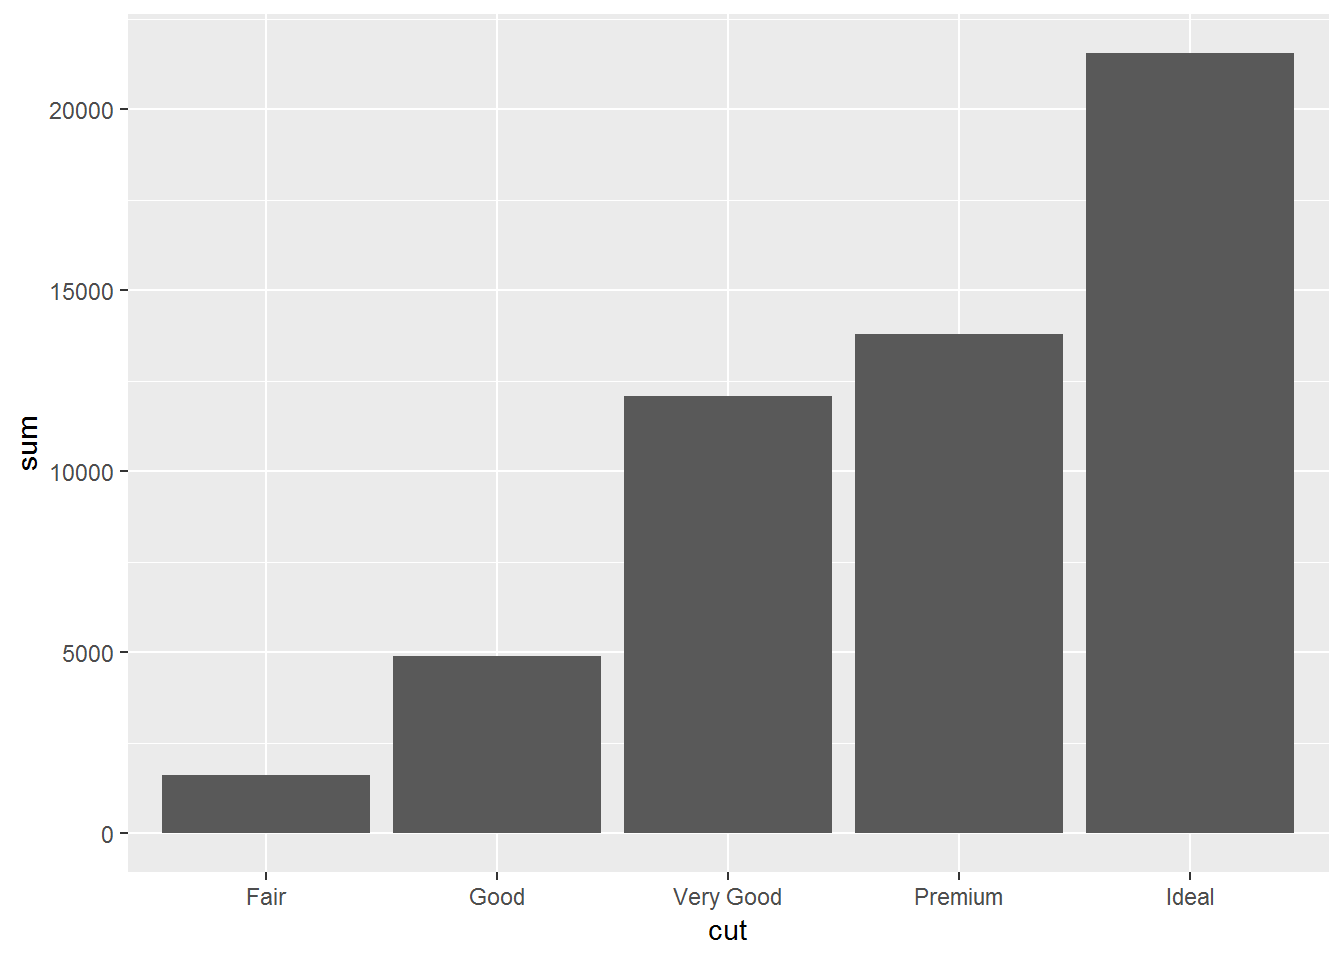
\includegraphics{jbm_files/figure-latex/unnamed-chunk-8-1.pdf}

\begin{enumerate}
\def\labelenumi{\arabic{enumi})}
\setcounter{enumi}{1}
\tightlist
\item
  cut에 따른 가격의 변화를 보여주는 그래프를 작성하세요.
\end{enumerate}

\begin{Shaded}
\begin{Highlighting}[]
\NormalTok{data8 <-}\StringTok{ }\KeywordTok{select}\NormalTok{(data6, cut, price) }\OperatorTok
\StringTok{  }\KeywordTok{group_by}\NormalTok{(cut) }\OperatorTok
\StringTok{  }\KeywordTok{summarise}\NormalTok{(}\DataTypeTok{price_mean1 =} \KeywordTok{mean}\NormalTok{(price))}

\KeywordTok{ggplot}\NormalTok{(data8, }\KeywordTok{aes}\NormalTok{(}\DataTypeTok{x=}\NormalTok{cut,}\DataTypeTok{y=}\NormalTok{price_mean1,}\DataTypeTok{group=}\DecValTok{1}\NormalTok{)) }\OperatorTok{+}
\StringTok{  }\KeywordTok{geom_bar}\NormalTok{(}\DataTypeTok{stat=}\StringTok{'identity'}\NormalTok{)}
\end{Highlighting}
\end{Shaded}

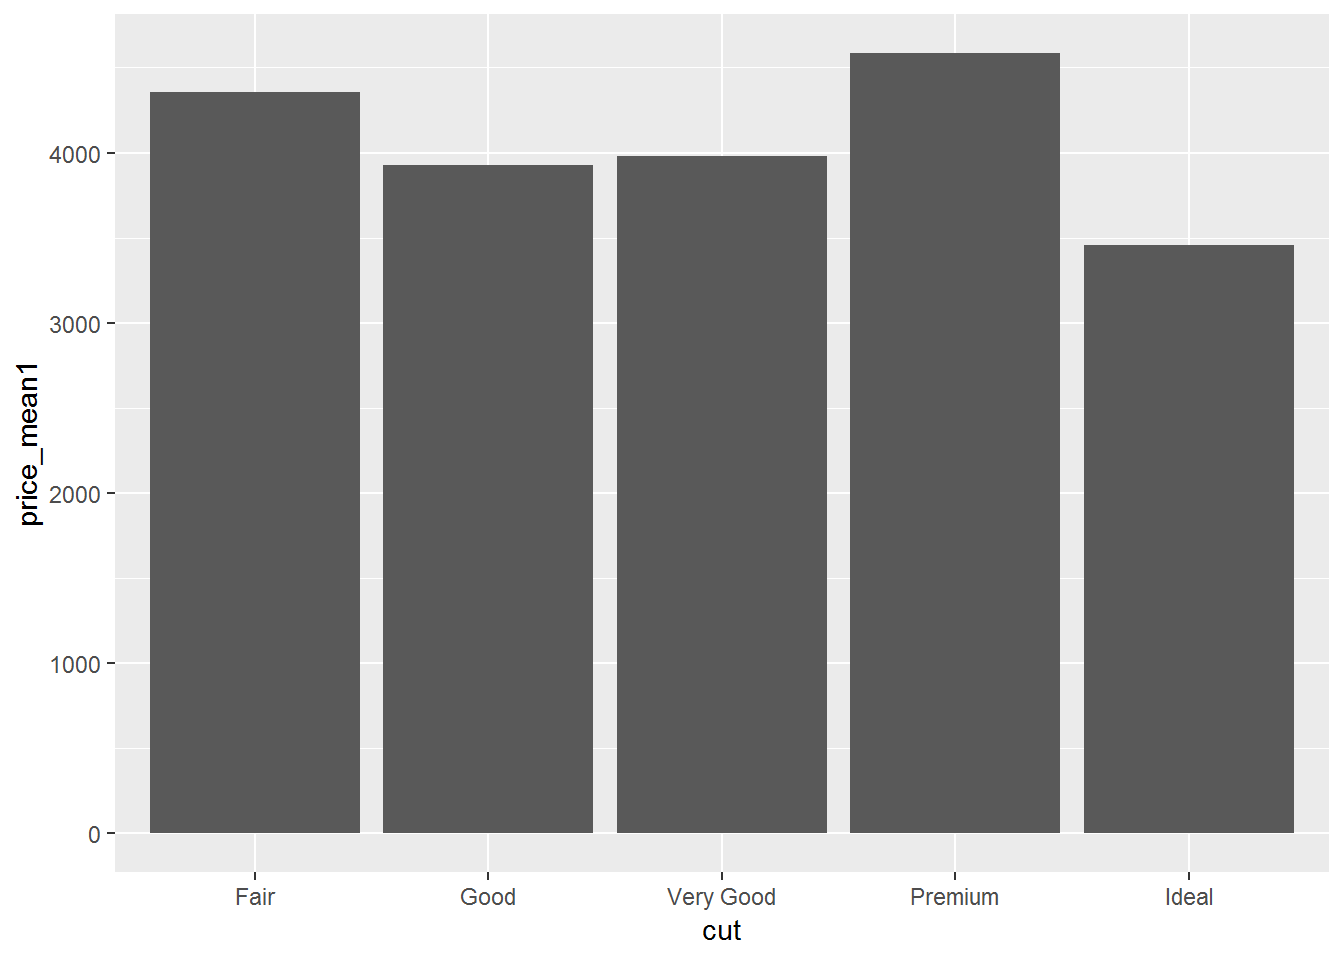
\includegraphics{jbm_files/figure-latex/unnamed-chunk-9-1.pdf}

\begin{enumerate}
\def\labelenumi{\arabic{enumi})}
\setcounter{enumi}{2}
\tightlist
\item
  cut과 color에 따른 가격의 변화를 보여주는 그래프를 작성하세요.
\end{enumerate}

\begin{Shaded}
\begin{Highlighting}[]
\NormalTok{data8 <-}\StringTok{ }\KeywordTok{select}\NormalTok{(data6, cut, price) }\OperatorTok
\StringTok{  }\KeywordTok{group_by}\NormalTok{(cut) }\OperatorTok
\StringTok{  }\KeywordTok{summarise}\NormalTok{(}\DataTypeTok{price_mean1 =} \KeywordTok{mean}\NormalTok{(price))}

\NormalTok{data9 <-}\StringTok{ }\KeywordTok{select}\NormalTok{(data6, color, price) }\OperatorTok
\StringTok{  }\KeywordTok{group_by}\NormalTok{(color) }\OperatorTok
\StringTok{  }\KeywordTok{summarise}\NormalTok{(}\DataTypeTok{price_mean2 =} \KeywordTok{mean}\NormalTok{(price))}

\NormalTok{gg1 <-}\StringTok{ }\KeywordTok{ggplot}\NormalTok{(data8, }\KeywordTok{aes}\NormalTok{(}\DataTypeTok{x=}\NormalTok{cut,}\DataTypeTok{y=}\NormalTok{price_mean1,}\DataTypeTok{group=}\DecValTok{1}\NormalTok{)) }\OperatorTok{+}
\StringTok{  }\KeywordTok{geom_bar}\NormalTok{(}\DataTypeTok{stat=}\StringTok{'identity'}\NormalTok{)}

\NormalTok{gg2 <-}\StringTok{ }\KeywordTok{ggplot}\NormalTok{(data9, }\KeywordTok{aes}\NormalTok{(}\DataTypeTok{x=}\NormalTok{color,}\DataTypeTok{y=}\NormalTok{price_mean2,}\DataTypeTok{group=}\DecValTok{1}\NormalTok{)) }\OperatorTok{+}
\StringTok{  }\KeywordTok{geom_bar}\NormalTok{(}\DataTypeTok{stat=}\StringTok{'identity'}\NormalTok{)}
\end{Highlighting}
\end{Shaded}


\end{document}
